\documentclass[]{article}
\usepackage{lmodern}
\usepackage{amssymb,amsmath}
\usepackage{ifxetex,ifluatex}
\usepackage{fixltx2e} % provides \textsubscript
\ifnum 0\ifxetex 1\fi\ifluatex 1\fi=0 % if pdftex
  \usepackage[T1]{fontenc}
  \usepackage[utf8]{inputenc}
\else % if luatex or xelatex
  \ifxetex
    \usepackage{mathspec}
    \usepackage{xltxtra,xunicode}
  \else
    \usepackage{fontspec}
  \fi
  \defaultfontfeatures{Mapping=tex-text,Scale=MatchLowercase}
  \newcommand{\euro}{€}
\fi
% use upquote if available, for straight quotes in verbatim environments
\IfFileExists{upquote.sty}{\usepackage{upquote}}{}
% use microtype if available
\IfFileExists{microtype.sty}{%
\usepackage{microtype}
\UseMicrotypeSet[protrusion]{basicmath} % disable protrusion for tt fonts
}{}
\usepackage[margin=1in]{geometry}
\usepackage{graphicx}
\makeatletter
\def\maxwidth{\ifdim\Gin@nat@width>\linewidth\linewidth\else\Gin@nat@width\fi}
\def\maxheight{\ifdim\Gin@nat@height>\textheight\textheight\else\Gin@nat@height\fi}
\makeatother
% Scale images if necessary, so that they will not overflow the page
% margins by default, and it is still possible to overwrite the defaults
% using explicit options in \includegraphics[width, height, ...]{}
\setkeys{Gin}{width=\maxwidth,height=\maxheight,keepaspectratio}
\ifxetex
  \usepackage[setpagesize=false, % page size defined by xetex
              unicode=false, % unicode breaks when used with xetex
              xetex]{hyperref}
\else
  \usepackage[unicode=true]{hyperref}
\fi
\hypersetup{breaklinks=true,
            bookmarks=true,
            pdfauthor={Lisa MALIPHOL},
            pdftitle={Diateam: SCAD@COPS A Hybrid Network Intrusion Detection System},
            colorlinks=true,
            citecolor=blue,
            urlcolor=blue,
            linkcolor=magenta,
            pdfborder={0 0 0}}
\urlstyle{same}  % don't use monospace font for urls
\setlength{\parindent}{0pt}
\setlength{\parskip}{6pt plus 2pt minus 1pt}
\setlength{\emergencystretch}{3em}  % prevent overfull lines
\setcounter{secnumdepth}{0}

%%% Use protect on footnotes to avoid problems with footnotes in titles
\let\rmarkdownfootnote\footnote%
\def\footnote{\protect\rmarkdownfootnote}

%%% Change title format to be more compact
\usepackage{titling}
\setlength{\droptitle}{-2em}
  \title{Diateam: SCAD@COPS\\A Hybrid Network Intrusion Detection System}
  \pretitle{\vspace{\droptitle}\centering\huge}
  \posttitle{\par}
  \author{Lisa MALIPHOL}
  \preauthor{\centering\large\emph}
  \postauthor{\par}
  \predate{\centering\large\emph}
  \postdate{\par}
  \date{July 2015}




\begin{document}

\maketitle


~ ~

\begin{itemize}
\item
  Introduction

  \begin{itemize}
  \itemsep1pt\parskip0pt\parsep0pt
  \item
    Project background
  \item
    Problem definition
  \item
    Paper organization
  \end{itemize}
\item
  SCADA Systems

  \begin{itemize}
  \itemsep1pt\parskip0pt\parsep0pt
  \item
    Terms

    \begin{itemize}
    \itemsep1pt\parskip0pt\parsep0pt
    \item
      ICS
    \item
      SCADA
    \item
      PLC
    \item
      RTU
    \item
      HMI
    \end{itemize}
  \item
    Traffic characterization
  \end{itemize}
\item
  Protocols

  \begin{itemize}
  \itemsep1pt\parskip0pt\parsep0pt
  \item
    TCP
  \item
    MODBUS/TCP
  \end{itemize}
\item
  Common Attacks on SCADA

  \begin{itemize}
  \itemsep1pt\parskip0pt\parsep0pt
  \item
    Command Injection
  \item
    Response Injection
  \item
    Denial of Service
  \end{itemize}
\item
  Intrusion Detection Systems

  \begin{itemize}
  \itemsep1pt\parskip0pt\parsep0pt
  \item
    Host IDS
  \item
    Network IDS

    \begin{itemize}
    \itemsep1pt\parskip0pt\parsep0pt
    \item
      Signature-based
    \item
      Anomaly-based
    \end{itemize}
  \end{itemize}
\item
  Techniques of Network Intrusion Detection

  \begin{itemize}
  \itemsep1pt\parskip0pt\parsep0pt
  \item
    Statistical
  \item
    Machine Learning
  \item
    Data Mining
  \end{itemize}
\item
  Tools

  \begin{itemize}
  \itemsep1pt\parskip0pt\parsep0pt
  \item
    Wireshark
  \item
    TShark
  \item
    UNIX unitilites - sed, awk, bash, etc.
  \item
    R
  \item
    C++
  \item
    SQLite3/MySQL
  \end{itemize}
\item
  Data Source
\item
  Exploratory Data Analysis
\item
  Statistical Measures/Features
\item
  Architecture

  \begin{itemize}
  \itemsep1pt\parskip0pt\parsep0pt
  \item
    Process (Figure 1)

    \begin{itemize}
    \itemsep1pt\parskip0pt\parsep0pt
    \item
      Step 1: Data Acquisition During Normal Activity - From the IDS
      appliance, sniff the network traffic, extract and store data in a
      database.
    \item
      Step 2: Statistical Analysis

      \begin{itemize}
      \itemsep1pt\parskip0pt\parsep0pt
      \item
        2.1 - Process data - Perform any transformation, filtering and
        data cleansing necessary.
      \item
        2.2 - Calculate and determine statistical measures.
      \item
        2.3 - Configure appliance with statistical parameters.
      \end{itemize}
    \item
      Step 3: Detection Mode - Appliance is set to detection mode.
    \end{itemize}
  \item
    Technical Architecture (Figure 2)
  \end{itemize}
\end{itemize}

Figure 1 -
Process\\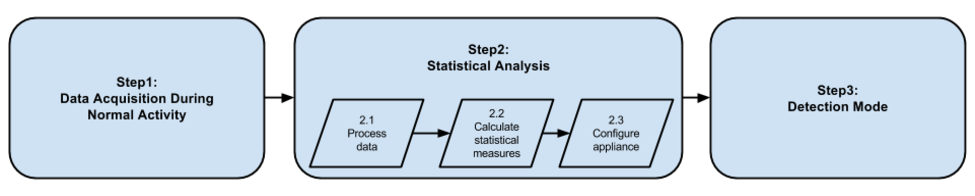
\includegraphics{reportOutline_files/figure-latex/unnamed-chunk-2-1.pdf}

Figure 2 - Technical
Architecture\\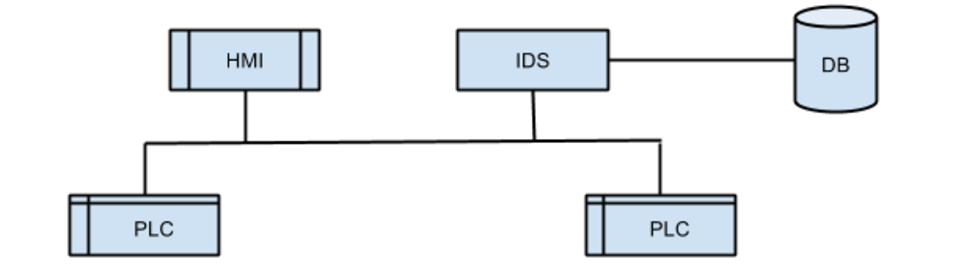
\includegraphics{reportOutline_files/figure-latex/unnamed-chunk-3-1.pdf}

\begin{itemize}
\item
  Implementation
\item
  Testing/Evaluation
\item
  Conclusion/Future Work
\item
  Bibliography
\item
  Appendices
\end{itemize}

\end{document}
